


%\pagebreak 

\section{Calibration} \label{sec: Calibration}
Table \ref{Table:Calibration} displays the parameters in the model and how they are chosen or calibrated. A large number of the parameters are calibrated in the steady state to match certain targets/statistics. For a reasonable amount of parameters, this can be done analytically.  
The main computational hurdle in the calibration lies in fitting the wealth distribution using the discount factors along with obtaining asset and labor market equilibria. In practice I calibrate all parameters that can be calibrated independently of the household problem first. This yields bonds and firm equity $B_{ss}, p^e_{ss}$, which through the mutual fond sum to aggregate household assets $A^{ss}$. I then minimize the following objective function:\footnote{After minimizing the objective function I apply a root finder to ensure exact asset market equilibrium by using the previous value of $\bar{\beta}$ from the minimization problem as starting value.}
\centerline{
  \begin{minipage}{\linewidth}
  \centering
\begin{align*}
\left[\left(B_{ss}+p_{ss}^{e}-A_{ss}^{*}\right)^{2}+\sum_{10,40,50}\left(\omega_{i}\left(\bar{\beta},\Delta^{\beta},\gamma^{\beta}\right)-\omega_{i}\right)^{2}+\left(\frac{\int_{\underline{a}}^{0}ad\mathcal{D}_{ss}}{A_{ss}}-0.15\right)^{2} \right]
\end{align*}
\end{minipage}}


\vspace{0.7cm}
The first term ensures asset market equilibrium. This is primarily targeted with $\bar{\beta}$. The second term fits the wealth distribution to the observed distribution in the data. In particular, it matches the share of wealth held by the bottom 10\%, the bottom 50\%, and the middle 40\%. These moments are "targeted" with the dispersion of discount factors in the population $\Delta^{\beta}$ and the distribution parameter $\gamma^{\beta}$.\footnote{Discount factors are distributed according to $\mathcal{D}^{\beta}=\left\{ d_{1}^{\beta},d_{2}^{\beta},...,d_{n^{\beta}}^{\beta}\right\}$ where $d_{j}^{\beta}$ is the share of population with associated discount factor $\beta_j$ in $\beta=\left\{ \beta_{1},\beta_{2},...,\beta_{n^{\beta}}\right\}$. The weights are parametrized as $d_{j}^{\beta}=\frac{j^{\gamma^{\beta}}}{\sum_{j}j^{\gamma^{\beta}}}$ for $j=1,2,...,n^{\beta}$ such that $d^{\beta}=0$ implies that discount factors are uniformly distributed, $\gamma^{\beta}\rightarrow\infty$ implies that the entire population has the highest discount factor $\beta_{n^{\beta}}$ and so forth.}\footnote{This is what \citet{carroll2009precautionary} denotes the impatience condition.} In practice $\Delta^{\beta}$ and $\gamma^{\beta}$ are poorly identified from each other, but including $\gamma^{\beta}$ has the advantage that if $\beta_{n^{\beta}}$ is close to the upper bound for convergence $1/(1+r)$ one can increase $\gamma^{\beta}$ to increase asset holdings since this increases the share of households with high discount factors. The last term set the borrowing limit $\underline{a}$ such that 15\% of households are in debt.  \\




\subsubsection*{Households.} I set the elasticity of intertemporal substitution $\sigma$ to $0.5$ (corresponding to a CRRA-parameter of 2), which is standard in the literature. The persistence parameter $\rho^e$ for the earnings process $e_t$ is picked from \citet{floden2001idiosyncratic} who estimates the earnings process for Sweden resulting in $\rho^e = 0.81^\frac{1}{4}=0.95$ at the quarterly level. The standard error is set to $0.7$ from the same source. This is between the estimates used in \citet{kaplan2018monetary}, \citet{auclert2018intertemporal} (roughly 0.94), and \citet{hagedorn2019fiscal}, \citet{gornemann2016doves} (roughly 0.2). Note that the choice of standard error has two effects in the model: It determines the dispersion of income (the income distribution) and how strong the precautionary savings channel is w.r.t earnings. The importance of the first channel is primarily through the implied wealth distribution which affects the distribution of MPCs. However, since I calibrate to the wealth distribution using discount factors anyway, this channel is less important, though a more realistic income distribution of course reduces the amount of dispersion needed in discount factors. Thus the primary difference is in the precautionary savings channel. The calibration of the household block results in a mean discount factor $\bar{\beta}$ of $ 0.978$ with dispersion $\Delta^\beta=0.011$. Figure \ref{fig:Beta_dist} plots the estimated density of discount factors in the population.  \\

%following \citet{kaplan2018monetary} (note though that this is based on American data!). The discretization results in a vector of states $e$ of size $n^e$, a stochastic transition matrix $\mathcal{D}^{e}$ of size $n^{e}\times n^{e}$. I let $\mathcal{D}^{e}\left(e^{i},e^{j}\right)$ denote the probability of transitioning from state $e^i$ to $e^j$. Iterating on the transition matrix yields the ergodic distribution vector $d^{e}$ (of size $1\times n^{e}$), where each entry is the share of households in state a particular state. Since the process has mean 1 we have $d^{e}\cdot e'=1$. \\

%I set the persistence of the earnings risk process to 0.82, which is the estimate for Sweden from \citet{floden2001idiosyncratic}. The standard deviation is set to $ 0.92$ as in \citet{kaplan2018monetary}, \citet{auclert2018inequality}, though this of course primarily reflects US earnings risk. The calibration of the household block results in a mean discount factor $\bar{\beta}$ of $ 0.978$ with dispersion $\Delta^\beta=0.011$. Figure \ref{fig:Beta_dist} plots the estimated density of discount factors in the population.  \\


\subsubsection*{Firms.} The output elasticity of capital $\alpha$ is set to $0.35$, which is standard. The steady-state markup is set to 1.1 which implies an elasticity of substitution of 11 in the underlying CES demand. The deprecation rate of capital is set to 6\% per year, $\delta^K=0.015$. Together with a steady-state interest rate of $0.5\%$ this pins the level of capital and the investment rate. The implied investment rate is 23\%, which is in accordance with an average investment rate of 21\% in the data from Statistics Denmark. I set the vacancy costs per hired worker equal to 7\% of the steady-state wage. This is consistent with the calibration in \citet{christiano2016unemployment} and evidence in \citet{silva2009labor}. 


\subsubsection*{Central Bank.} The steady state features zero inflation, $\pi_{ss} = 0, \Pi_{ss} = 1$. The steady-state interest and the central banks targeted interest rate $r^*$ is set to $0.5\%$ at the quarterly level. The coefficient on inflation in the Taylor rule $\phi^{MP}$ is set to a standard value of 1.3. For the smoothing parameter I set $\rho^{MP} = 0.8$.  


\subsubsection*{Government.} The relevant tax rates for the government are obtained from the data. This involves the standard VAT on consumer goods, corporate tax rates and the average income tax rates. I set the supply of government bonds $B$ to match the average government debt-to-gdp ratio of $40\%$ at a yearly frequency. Lumpsum taxes are used to satisfy the real government budget constraint. These are in turn distributed to households following a rule, which is estimated/calibrated to fit the danish pre- and post-tax income Gini coefficients of 0.44 and 0.25 respectively. The resulting transfer function is regressive, i.e. poorer households receive a larger share of government transfers. 
For the income tax rate, I fit a cubic spline to the average income tax rates obtained from the report \textit{Dansk Økonomi, efterår 2018} by the Danish Economic Council. Before fitting, I convert the income to percent of average income (39.000 DKK monthly for households in 2013 - see \citet{Indkomster2014DST}, Statistics Denmark). Figure \ref{fig:tax_function} displays the data and the fitted tax function. Above a threshold of 200\% of average income I impose a constant income tax rate of 46\%.  


\subsubsection{Labor Market.} \citet{hobijn2009job} estimates a job separation rate of $2\%$ at the monthly level for Denmark. I use this estimate, and set $\delta^L = 1- (1-0.02)^3 = 0.06$. I set the unemployment rate to 5\%. These two calibrations imply a steady-state job finding rate of 0.53, which is high compared with estimates from \citet{hobijn2009job} (27\% at the quarterly level). The probability of filling a vacancy (the matching probability) $m_t$ is set to 0.7 following \citet{den2000job} and \citet{ravenna2008vacancies}. The elasticity of the matching function $\xi$ is then set to satisfy the matching function. The resulting value is $\xi=1.4$, which is between the calibrated value of 1.27 in \citet{den2000job} and the 1.7 of \citet{gornemann2016doves}.  


\subsubsection{Business Cycle parameters.} The adjustment cost parameter of investments $\kappa_I$ is set to $6$ as in \citet{pedersen2013drives}. I choose the price adjustment cost parameter $\kappa_P$ to match a slope of 0.03 of the NK Philips curve. This slope is within the usual calibrations, and consistent with the empirical estimates from \citet{gali1999inflation}. This implies $\kappa_P = 11/0.03 = 366$. 



\begin{figure}[htb]
\makebox[\linewidth][c]{%
\centering
\begin{subfigure}{.5\textwidth}
  \centering
  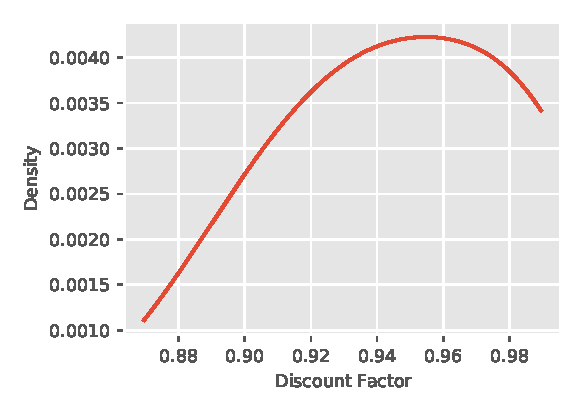
\includegraphics[width=.93\linewidth]{mainmatter/plots/SS_evaluation/Beta_density.pdf}
  \caption{Density of Discount factors.} \label{fig:Beta_dist}
\end{subfigure}%
\begin{subfigure}{.5\textwidth}
  \centering
  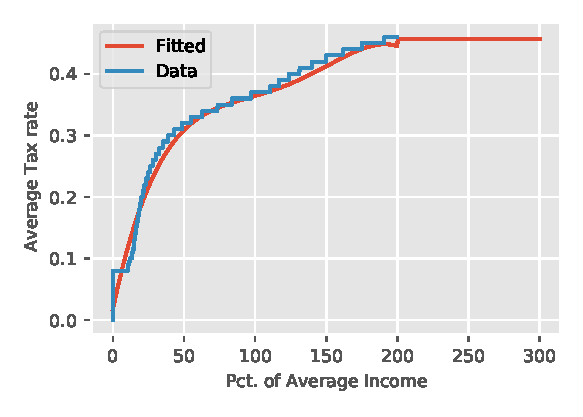
\includegraphics[width=.93\linewidth]{mainmatter/plots/SS_evaluation/tax_function1.pdf}
  \caption{Fitted tax function.} \label{fig:tax_function}
\end{subfigure}
}
\caption[Caption for LOF]{Calibrations}
\label{fig:SS_dists}
 \centering
  {\scriptsize  a) Kernel density of calibrated discount factors with average = 0.972. b) Tax function for average tax rates from the Danish Economic Council (\textit{Data}) and fit with cubic spline (\textit{Fitted}).}
\end{figure}




\bgroup
\def\arraystretch{1.0}
\setlength{\tabcolsep}{1.0em} 
\begin{table}[H]
\tiny
%\captionsetup{font=footnotesize}
\caption{Calibration} 
\label{Table:Calibration}
\centering
\footnotesize
\scalebox{0.9}{
\begin{threeparttable}
\scriptsize 
\makebox[\textwidth]{ 
\begin{tabular}{lcccc}
\toprule
\midrule
%\multicolumn{2}{c}{{Revenues}} & \multicolumn{2}{c}{Expenses} \\ 
 {Symbol}   & Desc.  & Value & Target  & Source  \\
 \cmidrule(lr){1-5}  
 
\multicolumn{5}{c}{\textbf{Households}} \\
\midrule
$\sigma$ & EIS & 0.5 & - & Standard \\ 
%$\varphi$ & Frisch Elasticity & 0.5 & - & Standard \\ 

%$\varphi$ & Disutility of labor & 0.01 & Job Finding rate = 30\% & \citet{hobijn2009job} \\ 
%$\varphi^{\ell}$ & Disutility of labor & 2.4 & $\int e_{i}\ell_{i}di=1$ & Calibrated \\ 

$\mu^\beta$ & Mean of Beta dist. & 0.93 & $r=0.5\%$ & Standard \\ 
$\Delta^\beta$ & Span of Beta dist. & 0.04 & Wealth Distribution Moments & \citet{balestra2018inequalities} \\ 
$\rho^\e$ & Persistence of earnings & 0.95 & - & \citet{floden2001idiosyncratic} \\ 
$\sigma^\e$ & SE of earnings & 0.7 & - & \citet{floden2001idiosyncratic} \\ 
$\kappa_{r^a}$ & Borrowing Wedge & $ 0.07 \cdot w_{ss}$ & 15\% of Households indebted  & \citet{kaplan2018monetary} \\ 
%\midrule
\multicolumn{5}{c}{} \\ 
\multicolumn{5}{c}{\textbf{Firms}} \\
\midrule
%$I$ & Investment rate & 0.22  & 22\% of GDP  & Statistics Denmark  \\ 
$\delta^K$ & Capital deprecation rate & 0.02  &   & Standard \\ 
%$I$ & SS Investment & 0.3  & 30\% of GDP  & Statistics Denmark  \\ 
$\kappa_P$ & Price Adj. Cost & 366  & NKPC slope = 0.03  & Standard  \\ 
$\kappa_I$ & Investment adjustment cost & 6  & -  & \citet{pedersen2013drives}  \\ 
$\kappa^V$ & Vacancy posting cost &  0.03 & $\frac{\kappa^{V}}{m}=0.07w^{ss}$ & \citet{christiano2016unemployment} \\ 
$\Phi^{F}$ & Fixed Cost &  12\% of $Y_{ss}$ & Wealth-to-Income ratio = 600\% & \citet{NB_wealth} \\ 
%\midrule
\multicolumn{5}{c}{} \\ 
\multicolumn{5}{c}{\textbf{Labor Market}} \\
\midrule
$\xi$ & Matching Elasticity & 1.4 & Unemployment rate = 5\% & Statistics Denmark \\ 
$w^{ss}$  & Steady-state wage & 0.63 &  Matching Probability = 0.7  & \citet{christiano2016unemployment} \\
$\delta^N$ & Job Destruction Rate & 0.06  & -  & \citet{hobijn2009job} \\ 
$m_t$ & Matching Probability & 0.7  & -  & \makecell{\citet{den2000job}, \\ \citet{ravenna2008vacancies} }  \\ 
$\eta_t$ & Wage elasticity  & 0.01  & -  & -  \\ 
\multicolumn{5}{c}{} \\ 
\multicolumn{5}{c}{\textbf{Government}} \\
%\multicolumn{5}{c}{} \\ 
\midrule
%$\tau^{VAT}$ & VAT & 0.25 &  -  &  Statutory Rate   \\
%$\tau^c$ & Corporate Tax rate & 0.22 &  -  &  Statutory Rate   \\
%$\tau^{div}$ & Dividend Tax rate & 0.42 &  -  &  Statutory Rate   \\
$G$  & Public Consumption & 0.24 &  24\% of GDP  & Statistics Denmark   \\
$B$  & Public Debt & 1.15 of $Y$ &  50\% of $A$  & Statistics Denmark   \\
%$\delta^{B}$  & Public Debt Maturity & 0.87 &  Maturity of 8 years  & \citet{NB_G}  \\
$b$  & Unemployment Benefits & 0.29 &  After tax Replacement rate of 51\% & \citet{schindler2011labor}  \\
$\phi^{\pi}$  & Inflation coefficient & 1.3 &  -  & Standard  \\
$\rho^{MP}$  & Interest rate smoothing & 0.8 &  -  & Standard  \\
\midrule[\heavyrulewidth]
\end{tabular}
}
\end{threeparttable}
}
%\begin{tablenotes}[para]\footnotesize 
%\item[1] The values for σ used in the literature are: 0.24 in Hall (2005a), 0.4 in Blanchard and Diamond (1989), Andolfatto
%(1994) and Merz (1995), 0.45 in Mortensen and Nagypal (2006), 0.5 in Hagedorn and Manovskii (2006), 0.5 in Farmer
%(2004), 0.72 in Shimer (2005a). See also a brief discussion in Mortensen and Nagypal (2006), p. 10, comparing their
%value of 0.45 to Shimer’s one \\
%\item[2] Labor Market Regulations in Low-, Middle- and High-Income Countries : A New Panel Database
%\end{tablenotes}
\end{table}




\subsection{Steady State Distributional Statistics}
Table \ref{table:Wealth_dist} shows how well the model fits the data in terms of the distribution of wealth. The targets (Middle 40\%, Bottom 50\%, Bottom 10\% and share of households in debt) all fit the data well, and by construction the top 10\% share of wealth also matches reasonably. The share of the top 1\% wealthiest is significantly underestimated, but this should have little implication for further analysis and is common to this type of model.0\footnote{To match the wealth share of the top wealthiest households entrepreneurial risk as in \citet{benhabib2014wealth} is usually needed.} The post-tax income Gini coefficient matches exactly the data, but given the minimal tax-transfer system the implied model pre-tax income Gini underestimates the data. 



\bgroup
\def\arraystretch{1.3}
%\setlength{\tabcolsep}{1.1em} 
\begin{table}[H] %\centering \footnotesize
\caption{Wealth Distribution - Model Fit vs. Data} \label{table:Wealth_dist}
\makebox[\textwidth]{ 
\begin{threeparttable}

\begin{tabular}{l*{2}{c}}
\hline\hline
\multicolumn{1}{c}{Share of Wealth of:}           & \multicolumn{1}{c}{Data} & \multicolumn{1}{c}{Model}    \\
%\multicolumn{1}{c}{Share of Wealth of:}           & \multicolumn{1}{c}{} & \multicolumn{1}{c}{}    \\
\hline 
Top 1\%     &  14.7\%  & 6.7\% \\  
Top 10\%    &  47.4\%  & 43.3\%  \\  
Middle 40\%   & 47.6\% & 51.7\% \\   
Bottom 50\%   & 5\% &  5\%  \\   
Bottom 10\% & -2.2\%  &  -2.4\% \\   
%Bottom 5\%  & -4.4\%  &    -4.4\% \\   
Share in debt & 15\%  & 16.4\% \\  
Share Constrained & -  & 0.9\% \\  
Wealth Gini    &  0.69 & 0.67 \\  
Income Gini (pre taxes \& transfers)   & 0.44   &   0.38  \\   
Income Gini (post taxes \& transfers)    & 0.25   & 0.31  \\   
\hline\hline 
\end{tabular}
  \begin{tablenotes}
     {\scriptsize See \citet{balestra2018inequalities} for all wealth distribution statistics. Gini coefficients for income are obtained from \citet{neamtu2014chapter}.} \\
    %\item[1] \scriptsize Negative values in the data, but given the borrowing constraint $\underline{a} = 0$ I impose that these targets must be 0. 
  \end{tablenotes}
\end{threeparttable}
}
\end{table}


Table \ref{table:Household_dist_stat} displays characteristics across the wealth and income distributions respectively. Accumulated wealth exhibits a strong, positive correlation with the degree of patience $\beta$. This in turn implies a strong correlation with marginal propensities to consume, which are strongly decreasing in wealth across the population. The last two columns in panel A shows that the income distribution is off less importance in the determination of the wealth distribution. While there is a tendency for higher skill/earnings and lower unemployment rates as one move up the wealth ladder, the correlation is not monotone. In particular, the middle part of the distribution (the 30th-50th percentile range) have higher earnings on average compared to other parts of the distribution. This implies that high earnings can bring households to the middle of the distribution, but the movement further up the wealth ladder is determined primarily by the discount factor.
Panel B of the table shows similar statistics for the income distribution. The calibration implies a positive correlation between income (skill percentile) and MPCs, but not nearly as strong as for the wealth distribution. 
In steady-state unemployed households has on average 86\% the consumption of employed households. This is significantly less than the gap between wages and unemployment benefits of $51\%$, showing the effects of consumption smoothing across states.   
%which implies that the gap between wages and unemployment benefits has more than 1-for-1 pass-through onto consumption. 


\bgroup
\def\arraystretch{1.3}
%\setlength{\tabcolsep}{.8em} 
\setlength{\tabcolsep}{1.1em} 
%\renewcommand{\arraystretch}{2}
\begin{table}[H]%[H]
%\tiny 
%\scriptsize
\footnotesize
%\begin{threeparttable}
\caption{Distributional statistics for Households} \label{table:Household_dist_stat}
\makebox[\textwidth]{ 
\begin{threeparttable}
\begin{tabular}{l  cccc}

%\toprule
%\multicolumn{5}{c}{Panel A:}  \\
\multicolumn{5}{c}{Panel A: Wealth Distribution Characteristics} \\
\cline{1-5}
\multicolumn{1}{c}{} & \multicolumn{1}{c}{{MPC}} & \multicolumn{1}{c}{{Avg. $\beta$}} 
& \multicolumn{1}{c}{{Unemployment Rate}} & \multicolumn{1}{c}{{Skill Percentile}}  \\ 
\midrule
Top 1\%     &  0.02 & 0.994 & 5.01\%  & 94.8 \\  
Top 10\%    &  0.03 & 0.991 & 5.09\%  & 94.9 \\  
70th-90th   &  0.06 & 0.981 & 4.98\%  & 94.8  \\   
50th-70th   &  0.13 & 0.968 & 4.97\%  & 83.6 \\   
30th-50th   &  0.24 & 0.955 & 4.79\%  & 83.6 \\   
10th-30th   &  0.44 & 0.945 & 4.54\%  & 69.9 \\   
Bottom 10\% &  0.69 & 0.936 & 6.37\%  & 39.9  \\   
Bottom 1\%  &  0.99 & 0.937 & 2.13\%  & 63.9 \\   
\midrule
\midrule[\heavyrulewidth]
\end{tabular}
  \begin{tablenotes}
    {\scriptsize The table shows the average MPC, discount factor, unemployment rate and skill percentile for various groups in the wealth distribution. Top 1\% refers to the 1\% holding the most assets, and similarly for Top 10\%, Bottom 10\%, Bottom 1\%. 70th-90th refers to the group between the 70th percentile in the wealth distribution and the 90th percentile, and similarly for 50th-70th, 30th-50th, and 10th-30th.   }
  \end{tablenotes}
\end{threeparttable}

}
\makebox[\textwidth]{ 
\begin{threeparttable}
\begin{tabular}{l  ccc}
%\centering
\multicolumn{4}{c}{}  \\
%\multicolumn{4}{c}{Panel B:}  \\
\multicolumn{4}{c}{Panel B: Income Distribution Characteristics} \\
\cline{1-4} 
\multicolumn{1}{c}{} & \multicolumn{1}{c}{{MPC}} & \multicolumn{1}{c}{{Avg. Income Tax rate}} 
& \multicolumn{1}{c}{{Unemployment Rate}}   \\ 
\midrule
Top 1\%     &  0.06 & 46\% & 4.5\%  \\  
Top 10\%    &  0.09 & 46\% & 4.9\% \\  
70th-90th   &  0.18 & 45\% & 4.8\% \\   
50th-70th   &  0.25 & 37\% & 4.7\% \\   
30th-50th   &  0.29 & 30\% & 5\%  \\   
10th-30th   &  0.32 & 26\% & 5.8\%   \\   
Bottom 10\% &  0.32 & 11\% & 5.1\%   \\   
Bottom 1\%  &  0.23 & 8\% & 5.3\%  \\   
\midrule
\midrule[\heavyrulewidth]
\end{tabular}
  \begin{tablenotes}
     {\scriptsize Definitions are similar to those in panel A.}
  \end{tablenotes}
\end{threeparttable}
}
%{\raggedright\footnotesize\centering {Definitions are similar to those in panel A.} \par}

%\end{threeparttable}
 
\end{table}


  